\chapter{Разработка кроссплатформенного веб-приложения для визуализации численных данных}
\section{Цели и функциональность разрабатываемого приложения}
Конечная цель разрабатываемого приложения -- предоставить пользователям возможность загружать файлы и строить графики на основе данных, содержащихся в этих файлах. Для этого предусмотрена возможность загружать файлы различных форматов, имеющий табличное содержание, такие как CSV, Excel, Txt и другие.
После или до загрузки файла пользователю необхдимо выбрать тип и размерность графика, который он хочет построить, а также настроить параметры визуализации. Также желательно предусмотреть возможность навигации и масштабирования для возможности просмотреть в деталях необходимые участки. Разрабатываеоме приложение также предоставляет возможность сохранять графики в различных формате PNG.
Кроме того, благодаря концепциям реактивности и двустороннего связывания, имеется возможность сохранять настройки визуализации для повторного использования в пределах одной сессии, а также моментальный вывод графической информации. Это позволяет пользователям быстро создавать графики с теми же настройками, что они использовали ранее.
В целом, разрабатываемое приложение предоставляет широкий спектр функциональности для загрузки файлов, построения графиков и настройки визуализации. Основными причинами выбора данного набора функциональности является стремление сделать приложение максимально удобным и интуитивно понятным для людей не знакомых с программированием, чтобы они могли быстро и легко создавать красивые и информативные графики.
% \section{Информационная модель и архитектура приложения}
% Диаграммы классов, вариантов использования, компонентов, взаимодействия
\section{Описание выбранного набор технологий для разработки}
В ходе разработки программы были использованы различные технологии, собранные в единое веб-приложение для визуализации графической информации.

Основа разрабатываемого приложения -фрейморк Vue. Его парадигмы отлично подходят для разработки небольших проектов с мощным функционалом и современным интерфейсом. Основной концепцией, необходимой для отзывчивого взаимодействия с программой -- реактивность -- моментальное изменение состояния приложения при изменении вводимых данных. Она позволяет отображать графическую информацию в процессе изменения параметров визуализации для мгновенного получения информации об проведенном изменении пользователем.


Прототип интерфейса, описанный в главе 2 был переработан в векторном редакторе Figsadma (рисунок \ref{fig:11}). Перенос контекстного меню в правую часть отображения обусловлен передачей приоритета главного элемента блоку вывода графической информации. Основная идея создания области отображения визуализации с отношением сторон близким к 1:1 не притерпела изменений.
Также были добавлены конкретные кнопки и области для вывода различной информации. Цветовая схема была выбрана в зеленых тонах для создания ощущения когнитивной легкости и простоты использования инструментов приложения.



Как основа для визуализации была использована библиотека Plotly. Она дает наиболее разнообразный функционал и возможности для визуализации, но имеет слабо-структурированные настройки, что вызывало достаточно много глобальных проблем в процессе разработки. Однако результаты работы, а именно скорость отрисовки и качество графиков были на достаточно высоком уровне.
Для разработки использовалась среда WebStorm. Она значительно ускорила процесс обучения и разработки приложения. Также в нее была интегрирована система git, с помощью которой производилось управление кодом и версиями прграммы.

\begin{figure}[h!]
    \center
    
\includegraphics[scale=0.5]{fig/Figma.png}
    \caption{Интерфейс приложения, разработанный в редакторе Figma}
    \label{fig:11}
\end{figure}

В целом, использование этих технологий позволило создать удобное и функциональное приложение, которое должно удовлетворять потребностям пользователей.
% \section{Процесс разработки приложения}
% git репозиторий, комиты, пул-реквесты
\section{Тестирование разработанного программного обеспечения}
\subsection{Описание графического интерфейса пользователя}
Сформированный интерфейс не претерпел изменений в процес sсе разработки и сохранил основные черты макета, созданного в Figma (рисунок \ref{fig:12}). Кнопка <<Данные>> позволяет выбрать файл в котором должны содержаться данные табличного вида -- точки, расчитанные вне приложения, например с помощью различных программного обеспечения для обработки геоданных или программ для решения задач численных методов. При этом формат данных должен быть в виде построчной записи координат X, Y, Z с любым возможным разделителем. Выпадающие списки <<Размерность>> и <<Тип графика>> позволяют настроить параметры визуализации введенных данных, их содержимое описано в следующем пункте. Область <<Пример графика>> содержит изображение небольшого разрешения, взятого из официальной документации Plotly, которое визуализирует пример работы данного набора настроек. В области вывода графической информации также присутствуют всплывающие кнопки, помогающие в навигации и сохранении изображения в формате PNG.
\begin{figure}[h!]
    \center
    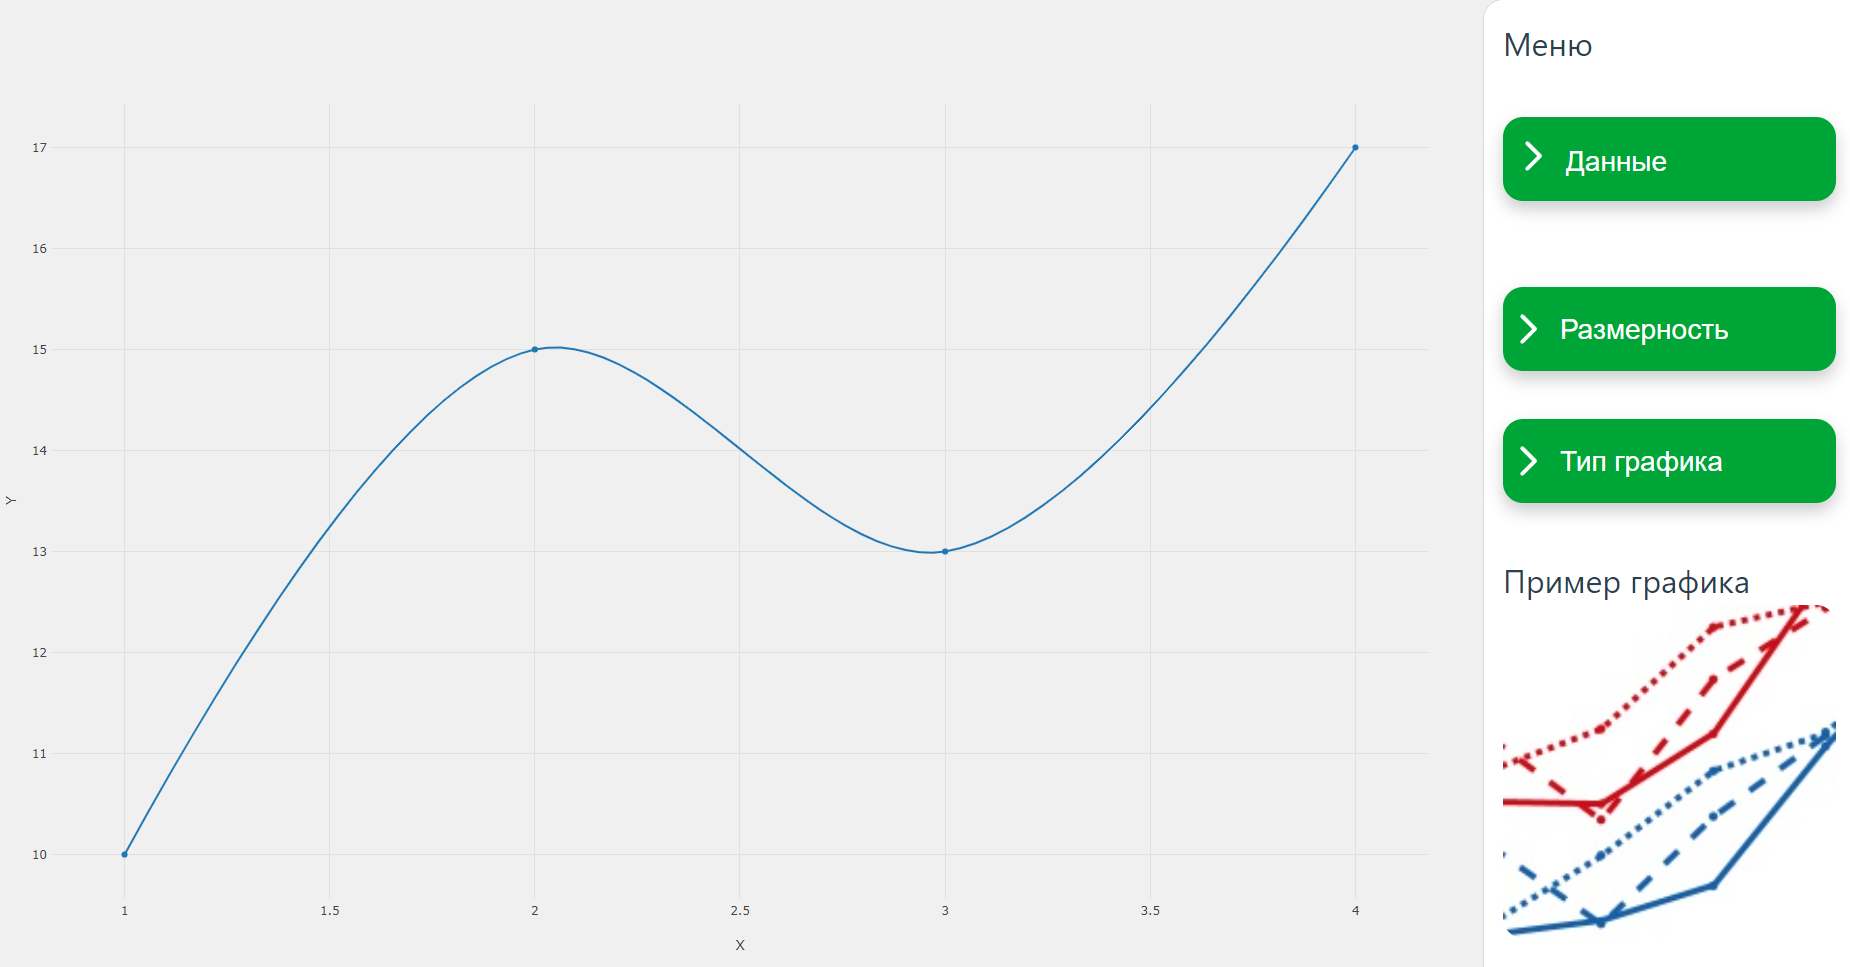
\includegraphics[scale=0.35]{fig/Interface.png}
    \caption{Интерфейс приложения, выполненный на Vue}
    \label{fig:12}
\end{figure}

\subsection{Варианты отображения графической информации и примеры работы}
С помощью выпадающего списка <<Размерность>> необходимо выбрать размерность вводимых данных: в трех измерениях или двух. В зависимости от размерности меняется содержимое выпадающего списка <<Тип графика>>. Для двумерного режима доступны опции:
\begin{enumerate}
    \item [1)] точечный график, изображенный на рисунке \ref{fig:13};
    \item [2)] линейный график, изображенный на рисунке \ref{fig:14};
    \item [3)] сплайн график, "изображенный на рисунке    " "  ;
    \item [4)] столбчатый график, изображенный на рисунке \ref{fig:16}. as as as sas 
\end{enumerate}

Данные опции никак не изменяют входные данные и используют их для отображения.
Для трехмерного режимо доступны опции:
\begin{enumerate} 
    \item [1)] точечный график, изображенный на рисунке \ref{fig:17};
    \item [2)] график изолиний, изображенный на рисунке \ref{fig:18};
    \item [3)] линейный график, изображенный на рисунке \ref{fig:19};
    \item [4)] объектный график, изображенный на рисунке \ref{fig:20};
    \item [5)] тепловая карта, изображенная на рисунке \ref{fig:21};
    \item [6)] график поверхности, изображенный на рисунке \ref{fig:22}.
\end{enumerate}


\newpage
\begin{figure}[h!]
    \center
    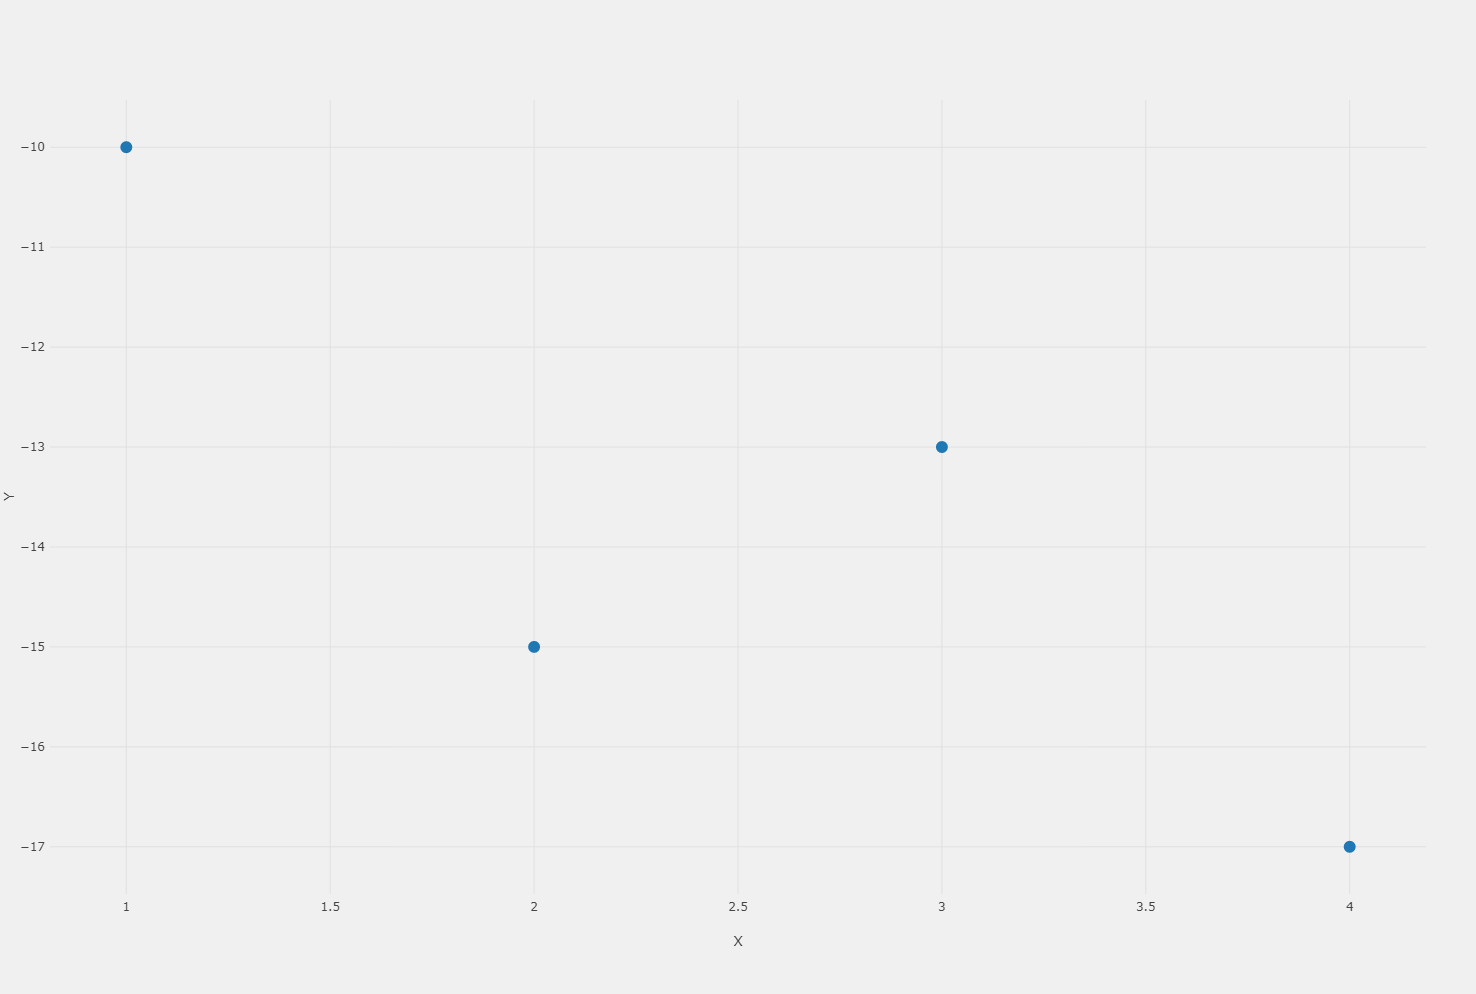
\includegraphics[scale=0.3]{fig/newplot (8).png}
    \caption{Пример точечного графика}
    \label{fig:13}
\end{figure}
\begin{figure}[h!]
    \center
    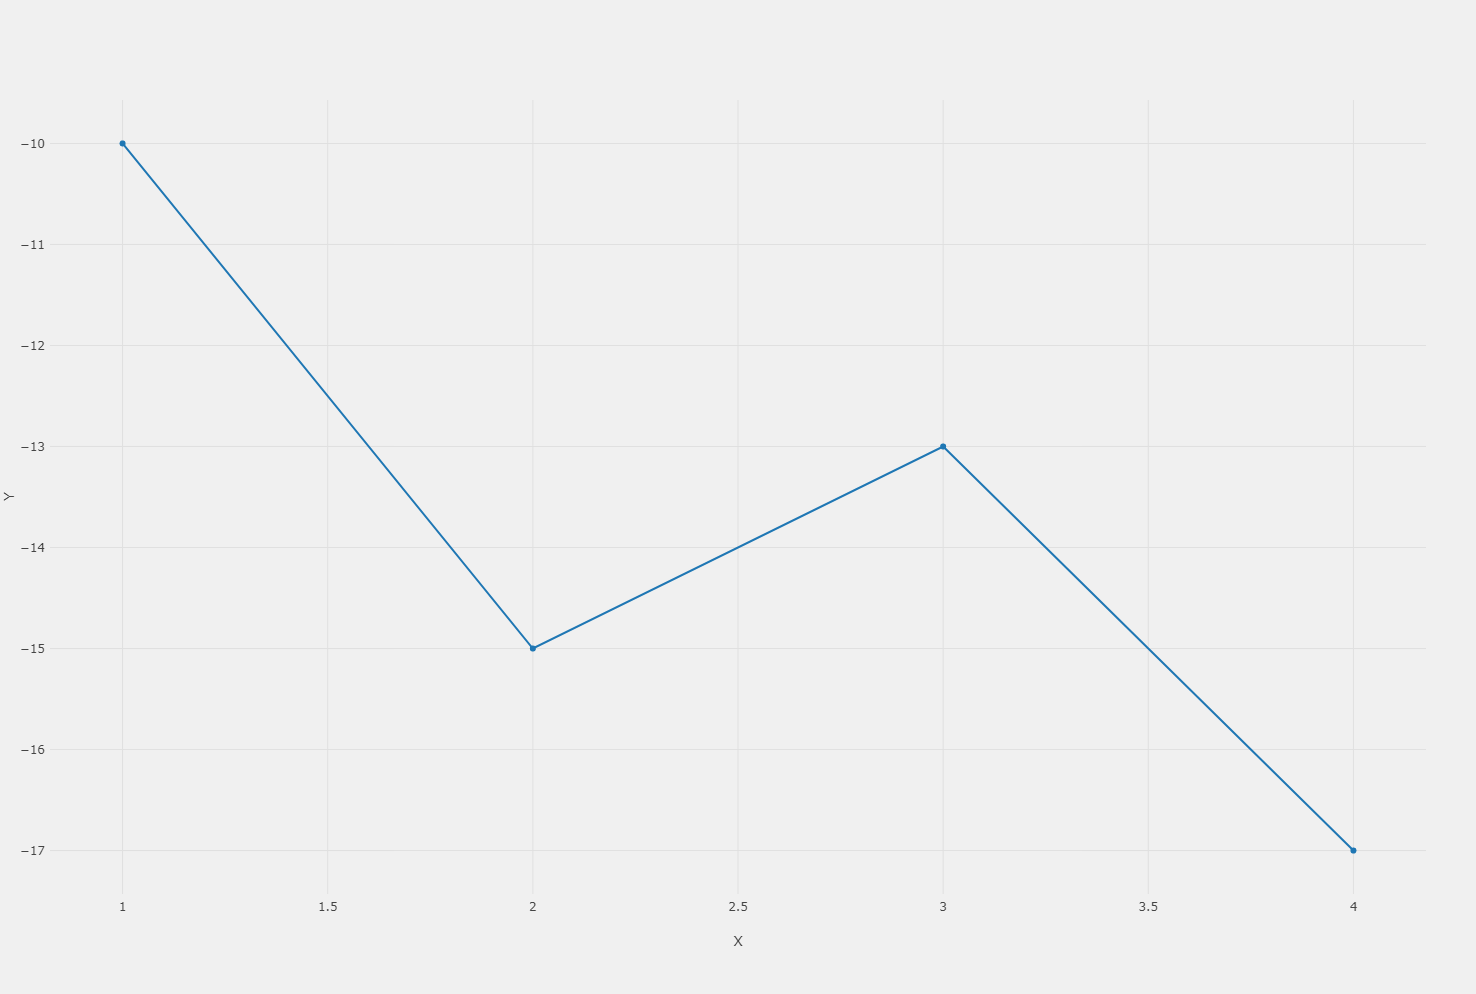
\includegraphics[scale=0.3]{fig/newplot (5).png}
    \caption{Пример линейного графика}
    \label{fig:14}
\end{figure}
\begin{figure}[h!]
    \center
    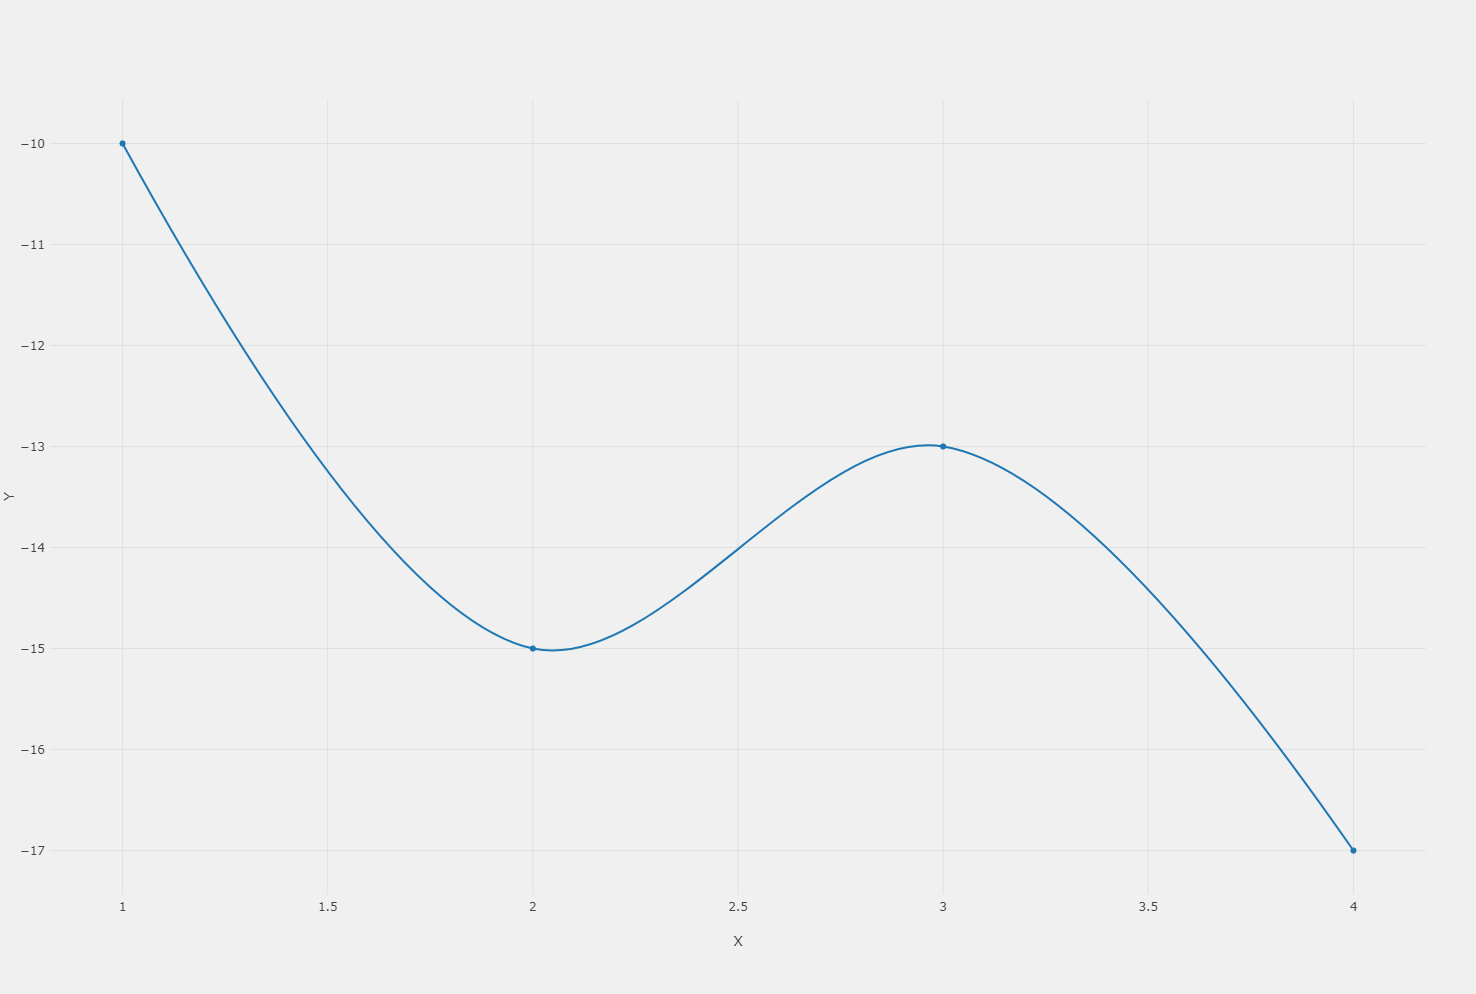
\includegraphics[scale=0.3]{fig/newplot (6).png}
    \caption{Пример сплайн графика}
    \label{fig:15}
\end{figure}
\begin{figure}[h!]
    \center
    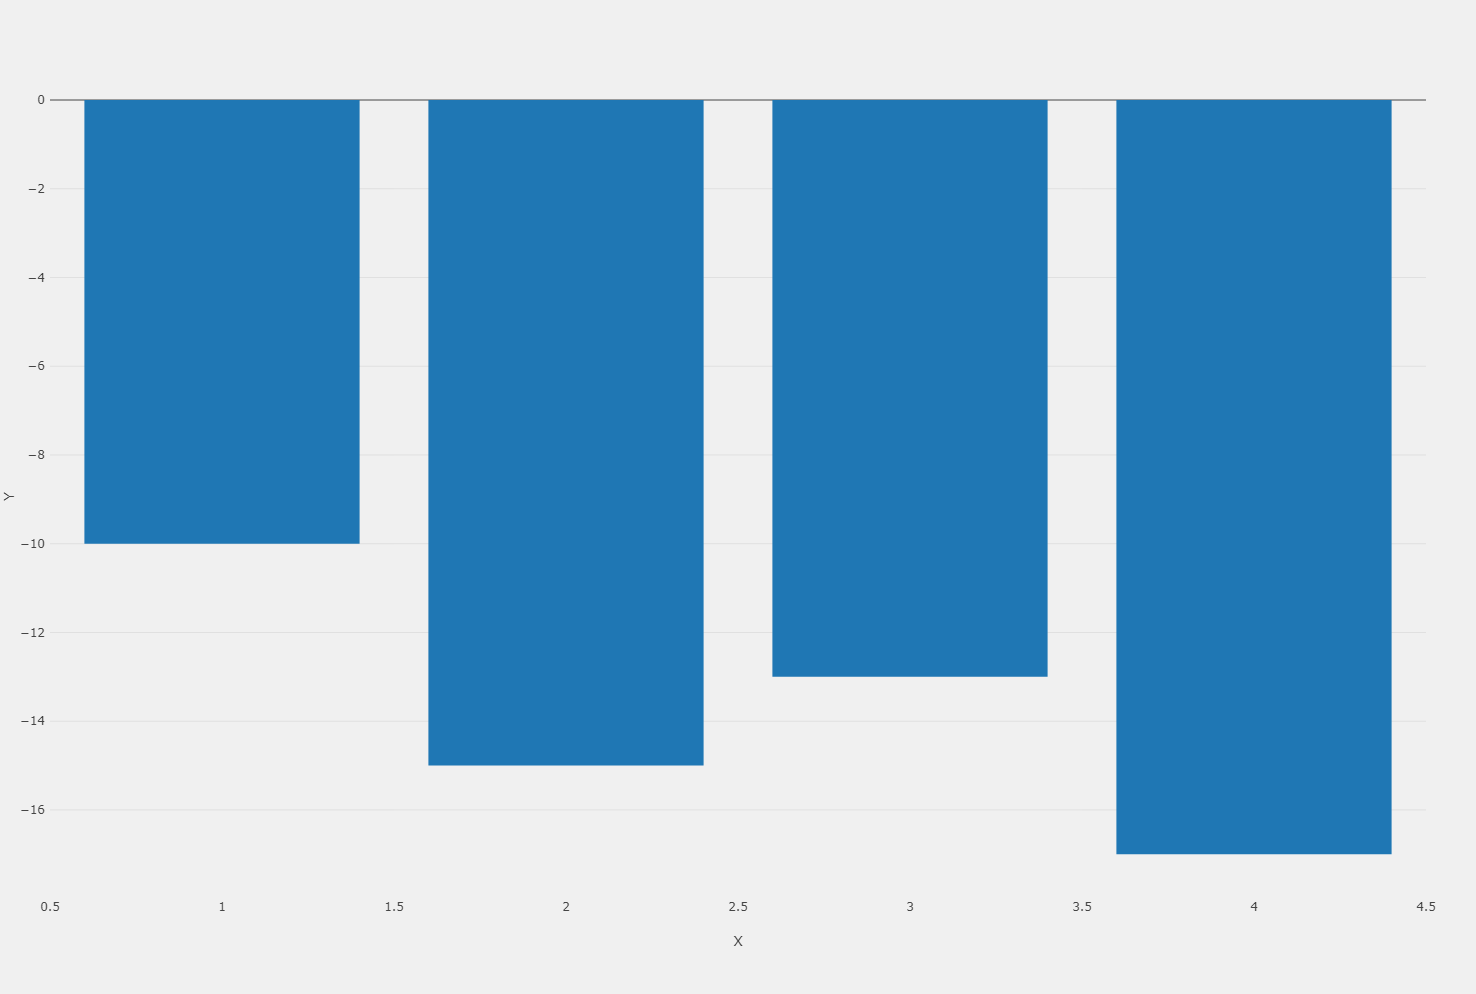
\includegraphics[scale=0.3]{fig/newplot (7).png}
    \caption{Пример столбчатого графика}
    \label{fig:16}
\end{figure}

\begin{figure}[h!]
    \center
    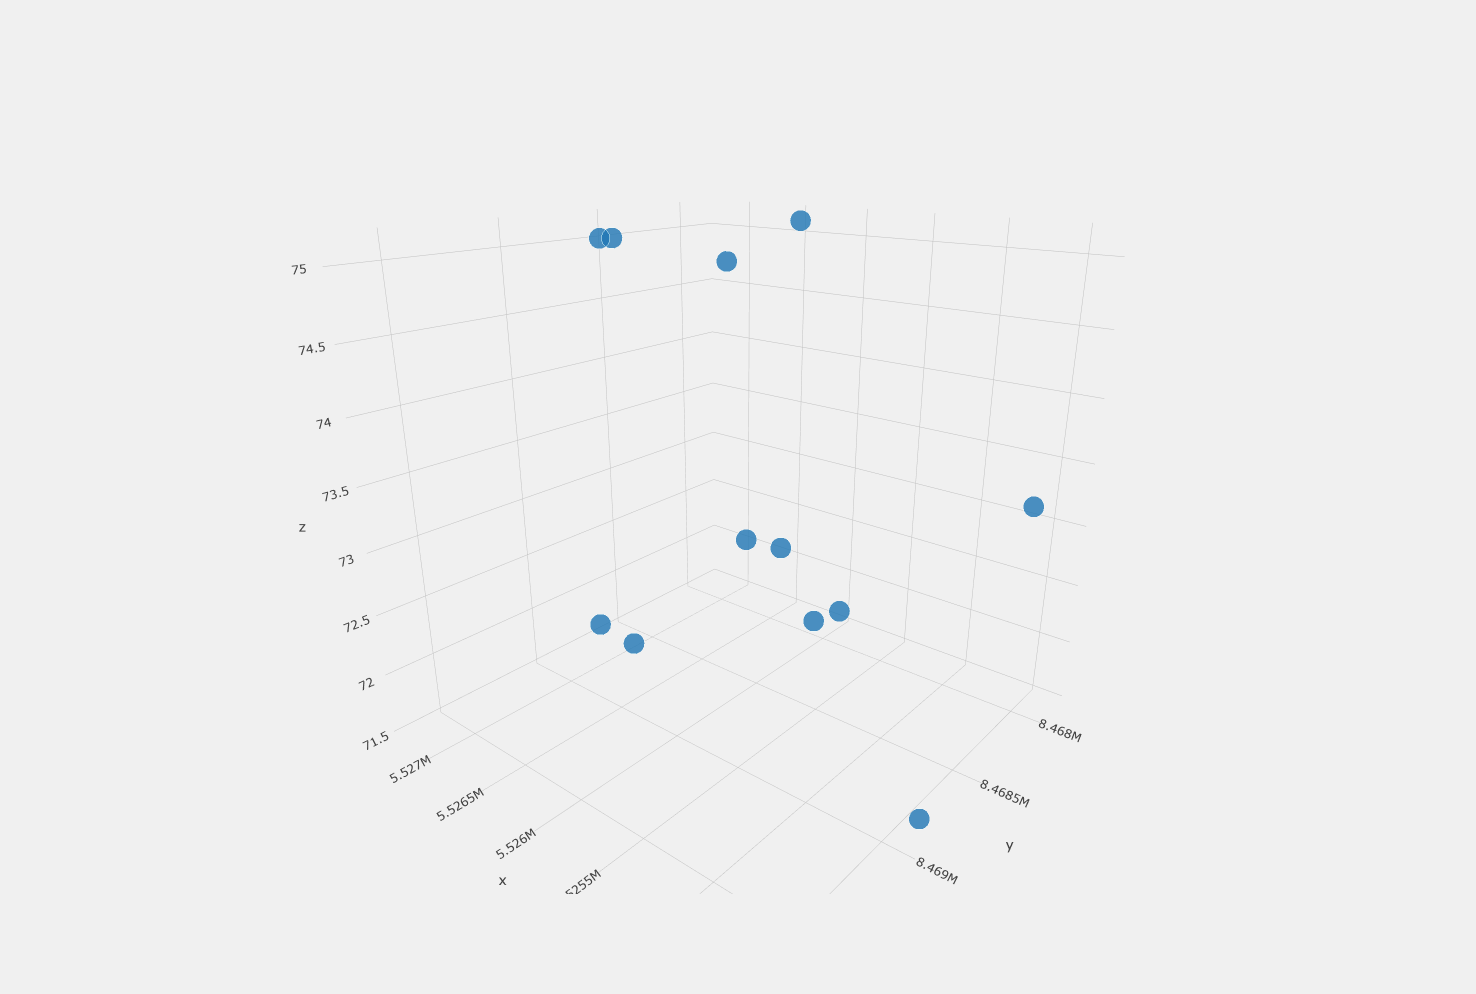
\includegraphics[scale=0.3]{fig/newplot (9).png}
    \caption{Пример точечного графика}
    \label{fig:17}
\end{figure}
\begin{figure}[h!]
    \center
    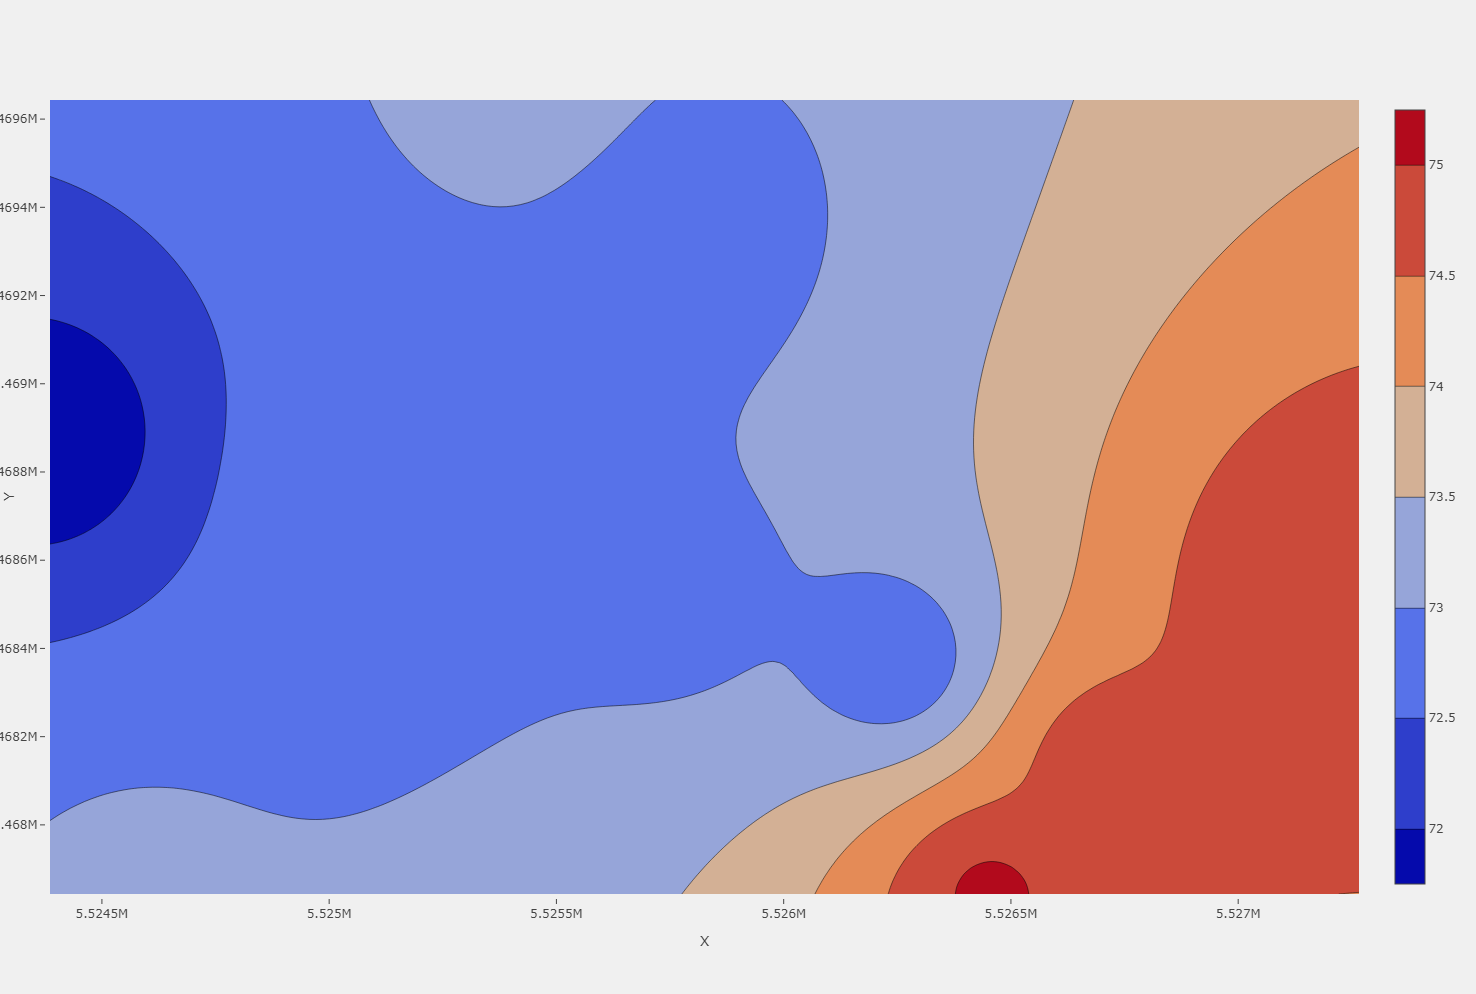
\includegraphics[scale=0.3]{fig/newplot (10).png}
    \caption{Пример графика изолиний}
    \label{fig:18}
\end{figure}
\begin{figure}[h!]
    \center
    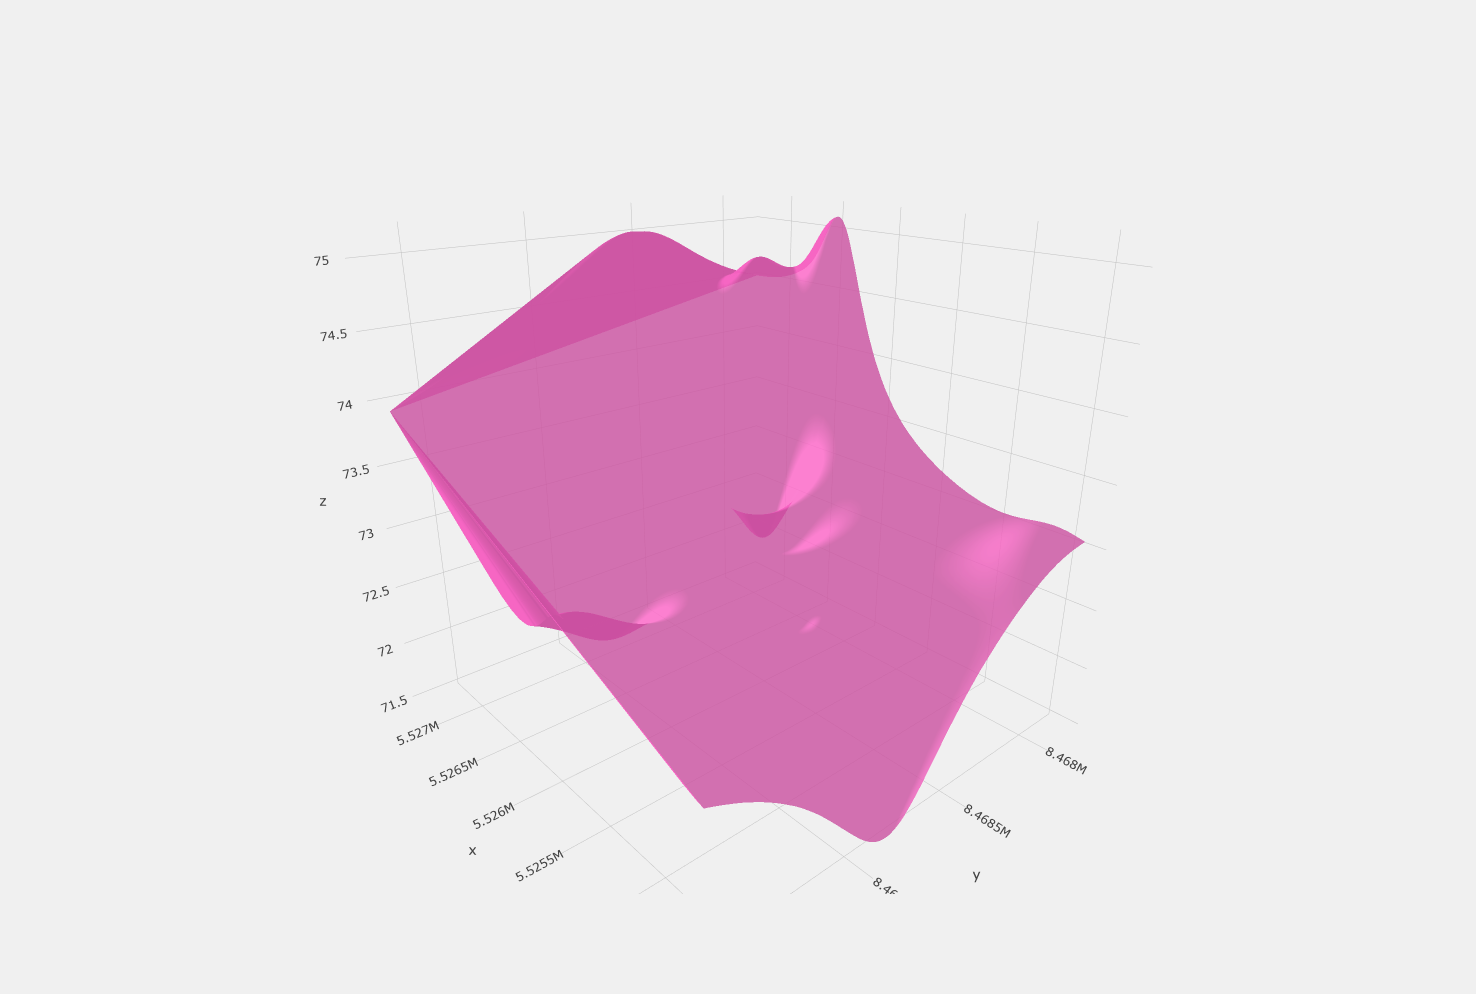
\includegraphics[scale=0.3]{fig/newplot (11).png}
    \caption{Пример линейного трехмерного графика}
    \label{fig:19}
\end{figure}
\begin{figure}[h!]
    \center
    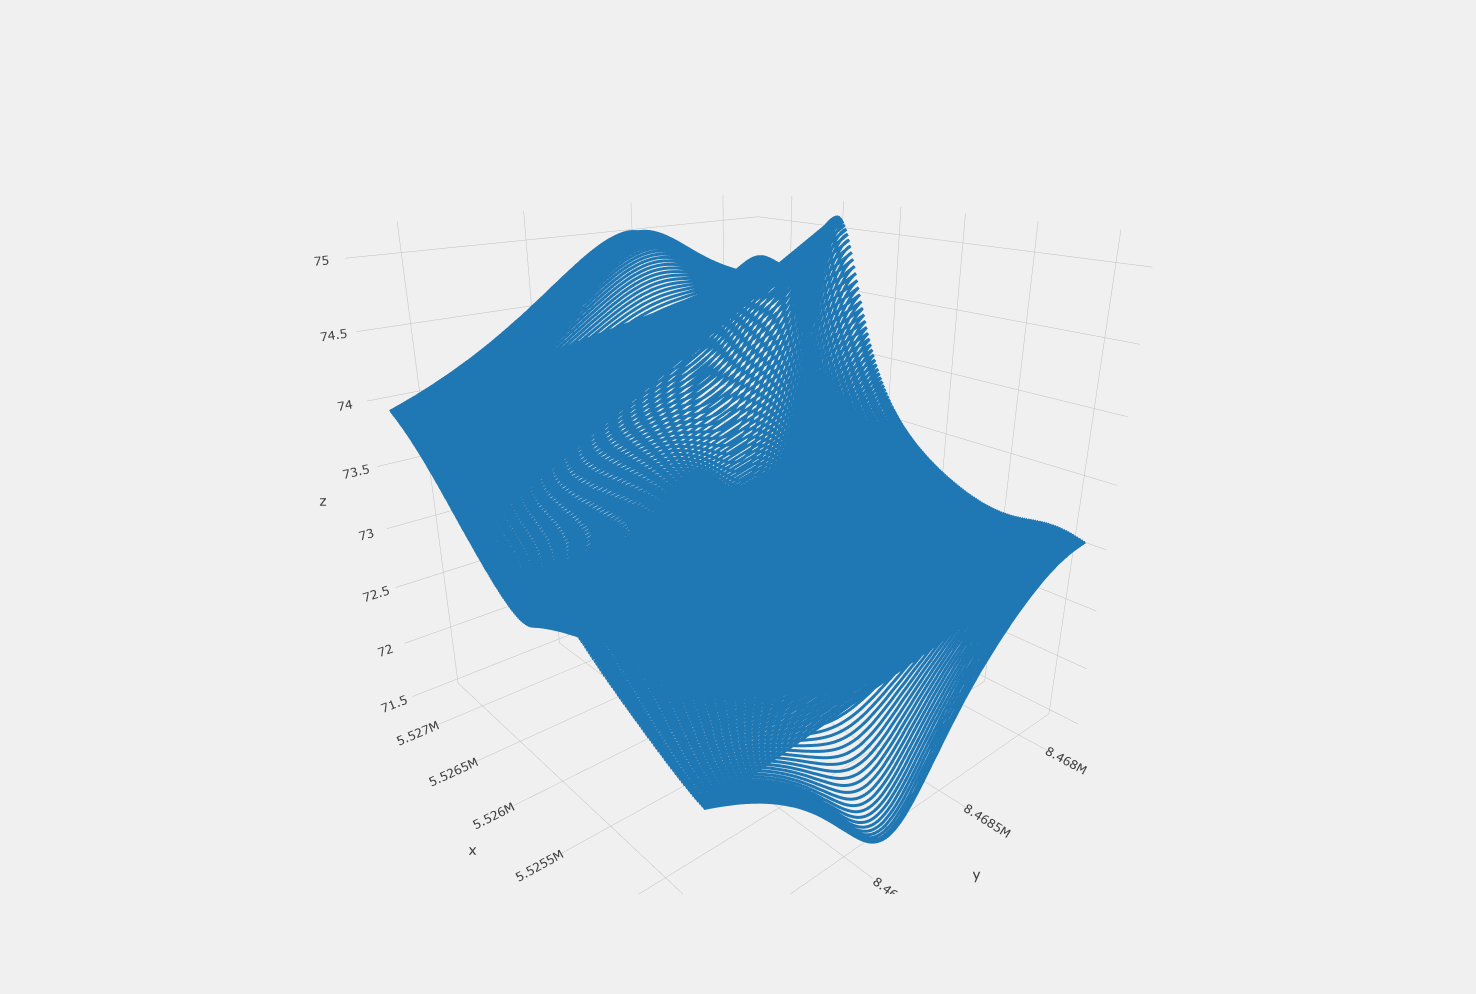
\includegraphics[scale=0.3]{fig/newplot (12).png}
    \caption{Пример объектного графика}
    \label{fig:20}
\end{figure}
\begin{figure}[h!]
    \center
    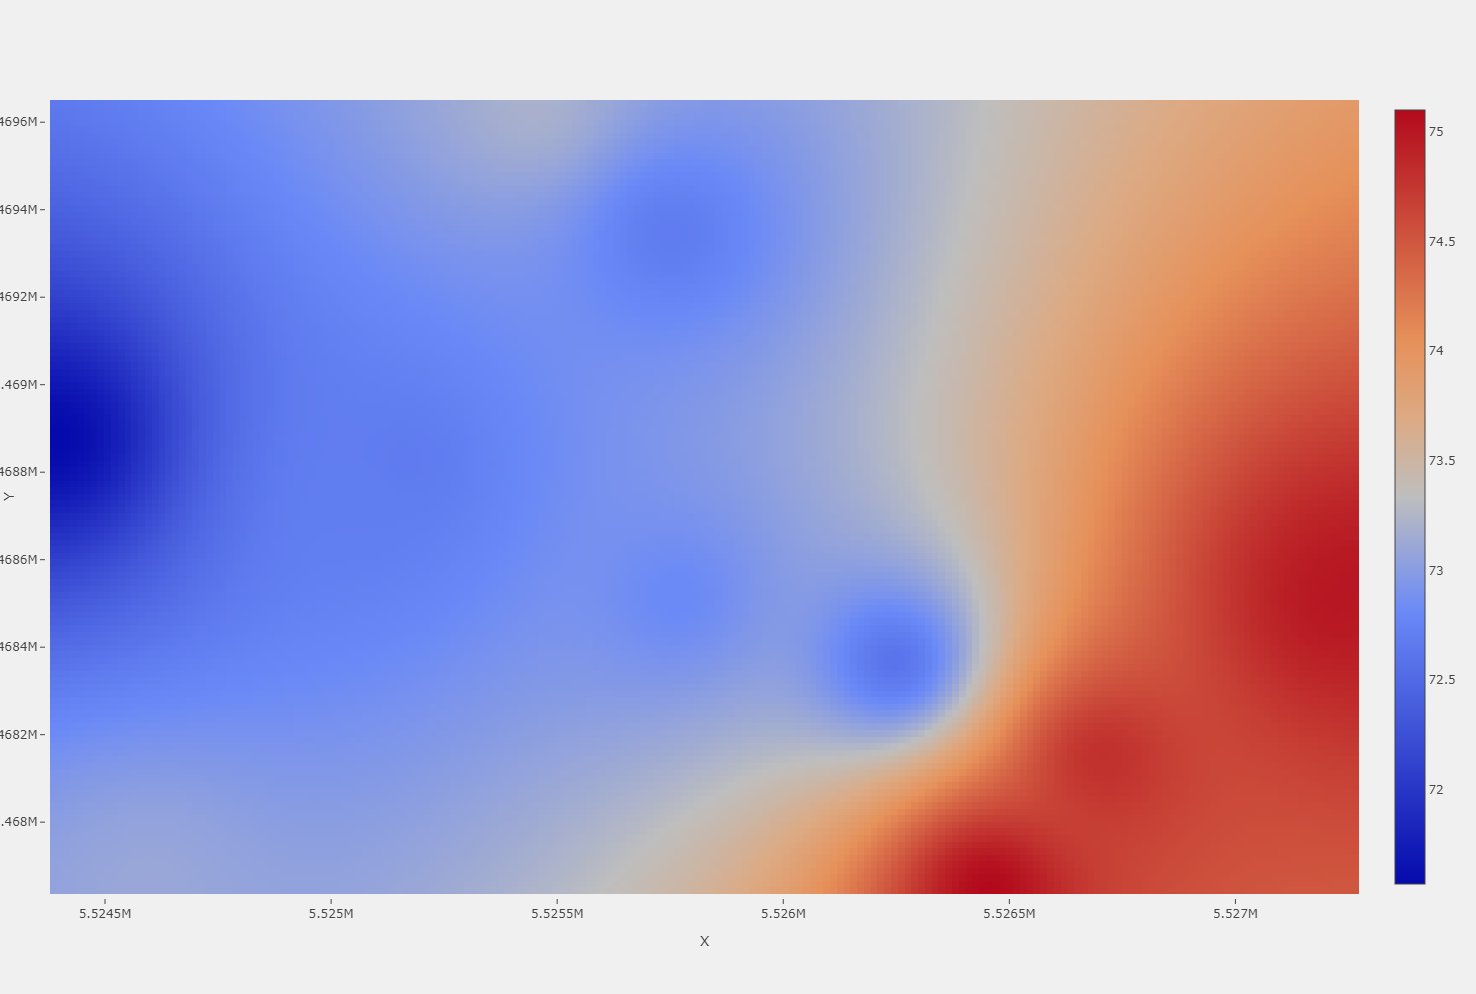
\includegraphics[scale=0.3]{fig/newplot (13).png}
    \caption{Пример тепловой карты}
    \label{fig:21}
\end{figure}
\begin{figure}[h!]
    \center
    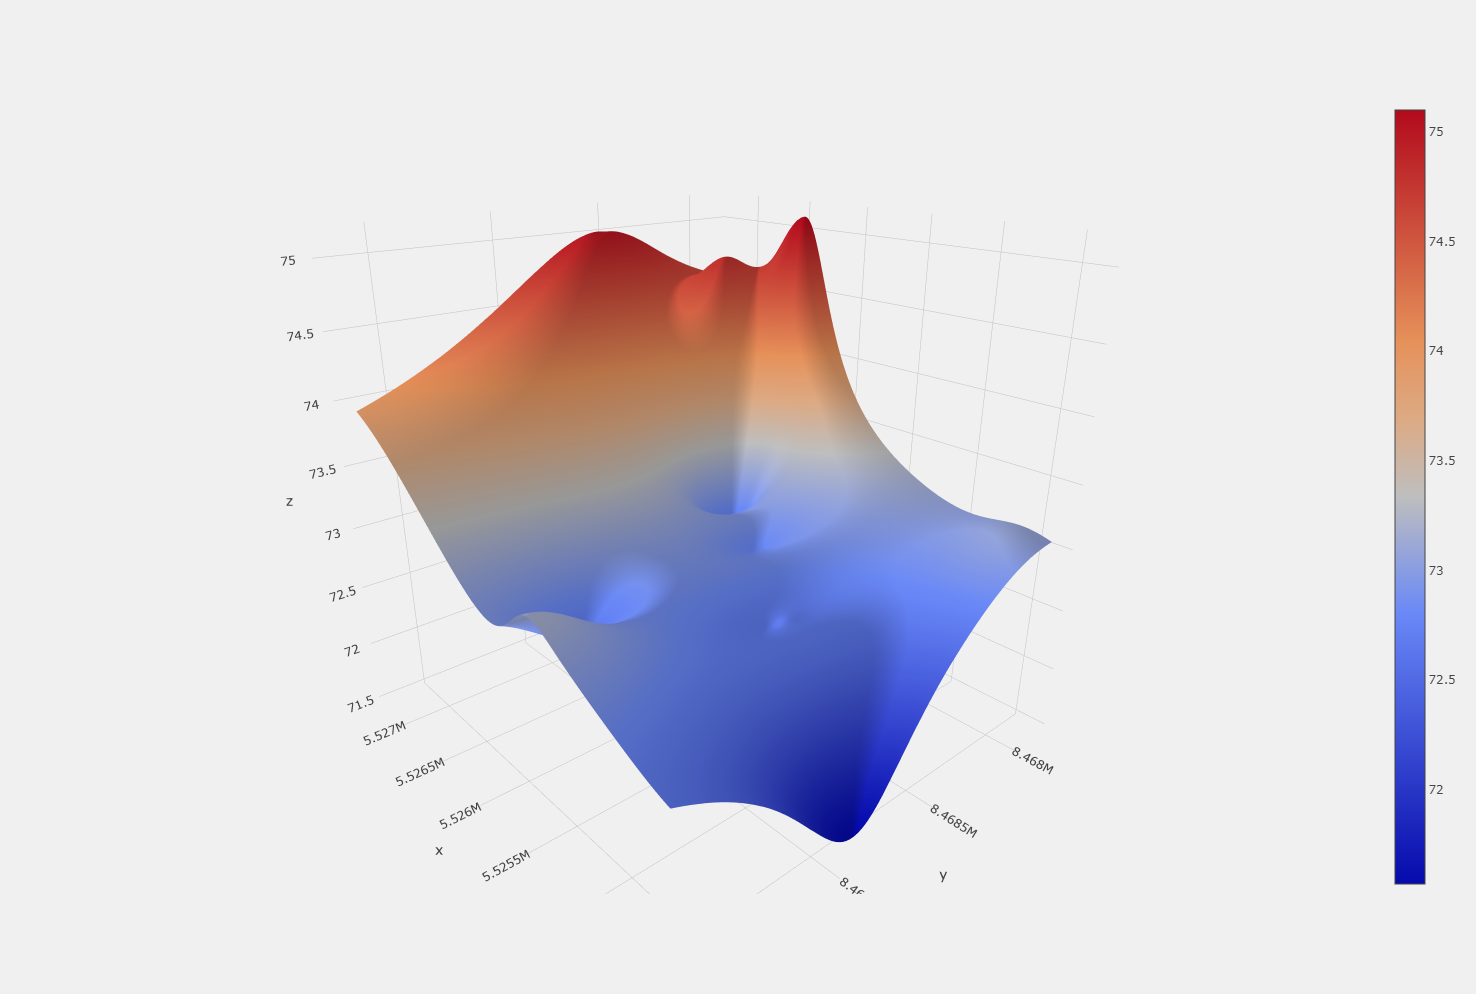
\includegraphics[scale=0.3]{fig/newplot (14).png}
    \caption{Пример поверхностного графика}
    \label{fig:22}
\end{figure}
% \subsection{Примеры работы приложения}
% Картинки и описание возможных поведений программы
\section{Сравнение с приложениями, имеющими сходный функционал}
Нижеприведенные программы имеют не только функционал, для визуализации числовых данных, но и дополнительный математические функции, которые, конечно, будут большим преимуществом при общем сравнении. Однако сравнительный анализ будет проведен только в области функциональности для отображения графической информации.

Программный пакет Advanced Grapher позволяет строить двумерные графики, поддерживает загрузку точек из файла, позволяет настроить стиль графика и маркеров, но не поддерживает выбор типа графиков и построение трехмерных графиков. Пример работы данного приложения указан на рисунке \ref{fig:23}. Также из-за устарелости интерфейса навигация по области отрисовки производится сложным и неудобным способом.

\begin{figure}[h!]
    \center
    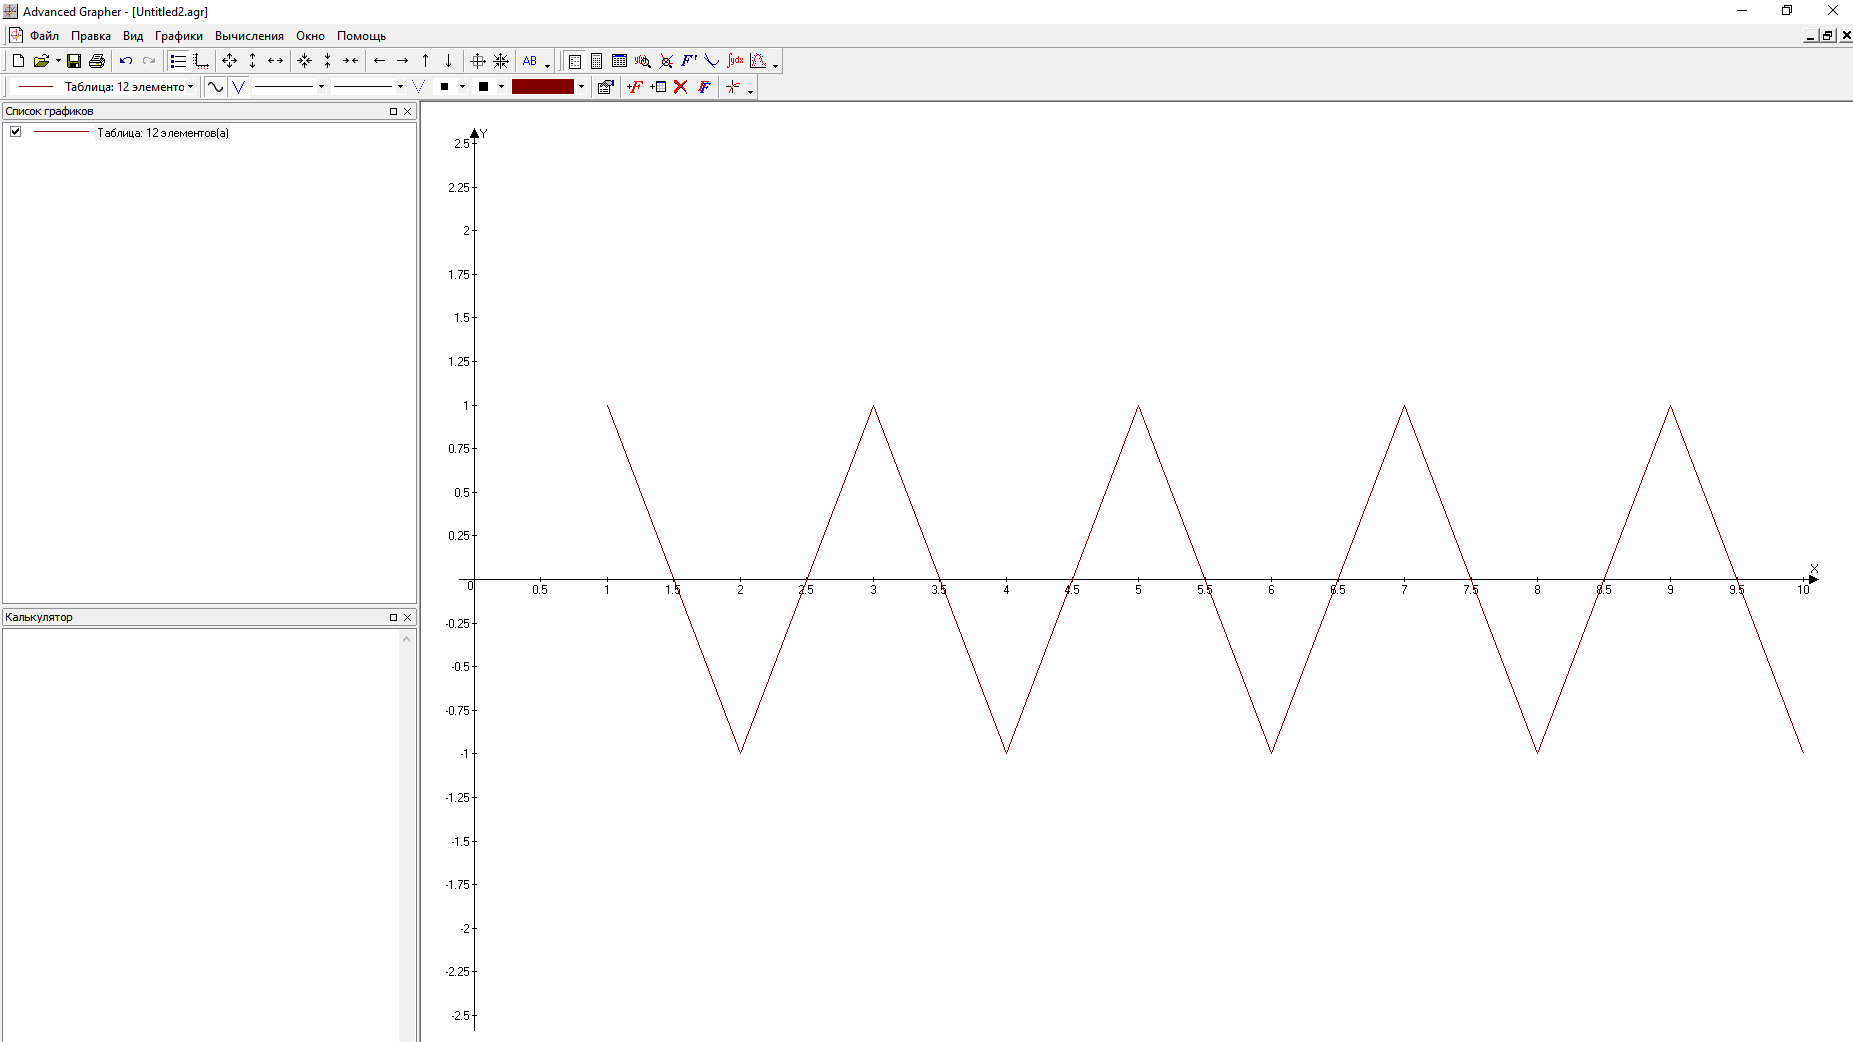
\includegraphics[scale=0.35]{fig/AdvancedGrapher.png}
    \caption{Пример работы программы Advanced Grapher}
    \label{fig:23}
\end{figure}

Приложение Geogebra не позволяет вводить табличные значения и работает только с аналитическими формулами, поддерживает как двумерную, так и трехмерную визуализацию, имеет современную систему навигации по области отрисовки, а также простой способ изменения стилей. Однако данное приложение не поддерживает графики изолиний, тепловые карты и не подходит, например, для анализа данных численного моделирования или геоданных. Пример работы данного приложения изображен на рисунке \ref{fig:24}.

\begin{figure}[h!]
    \center
    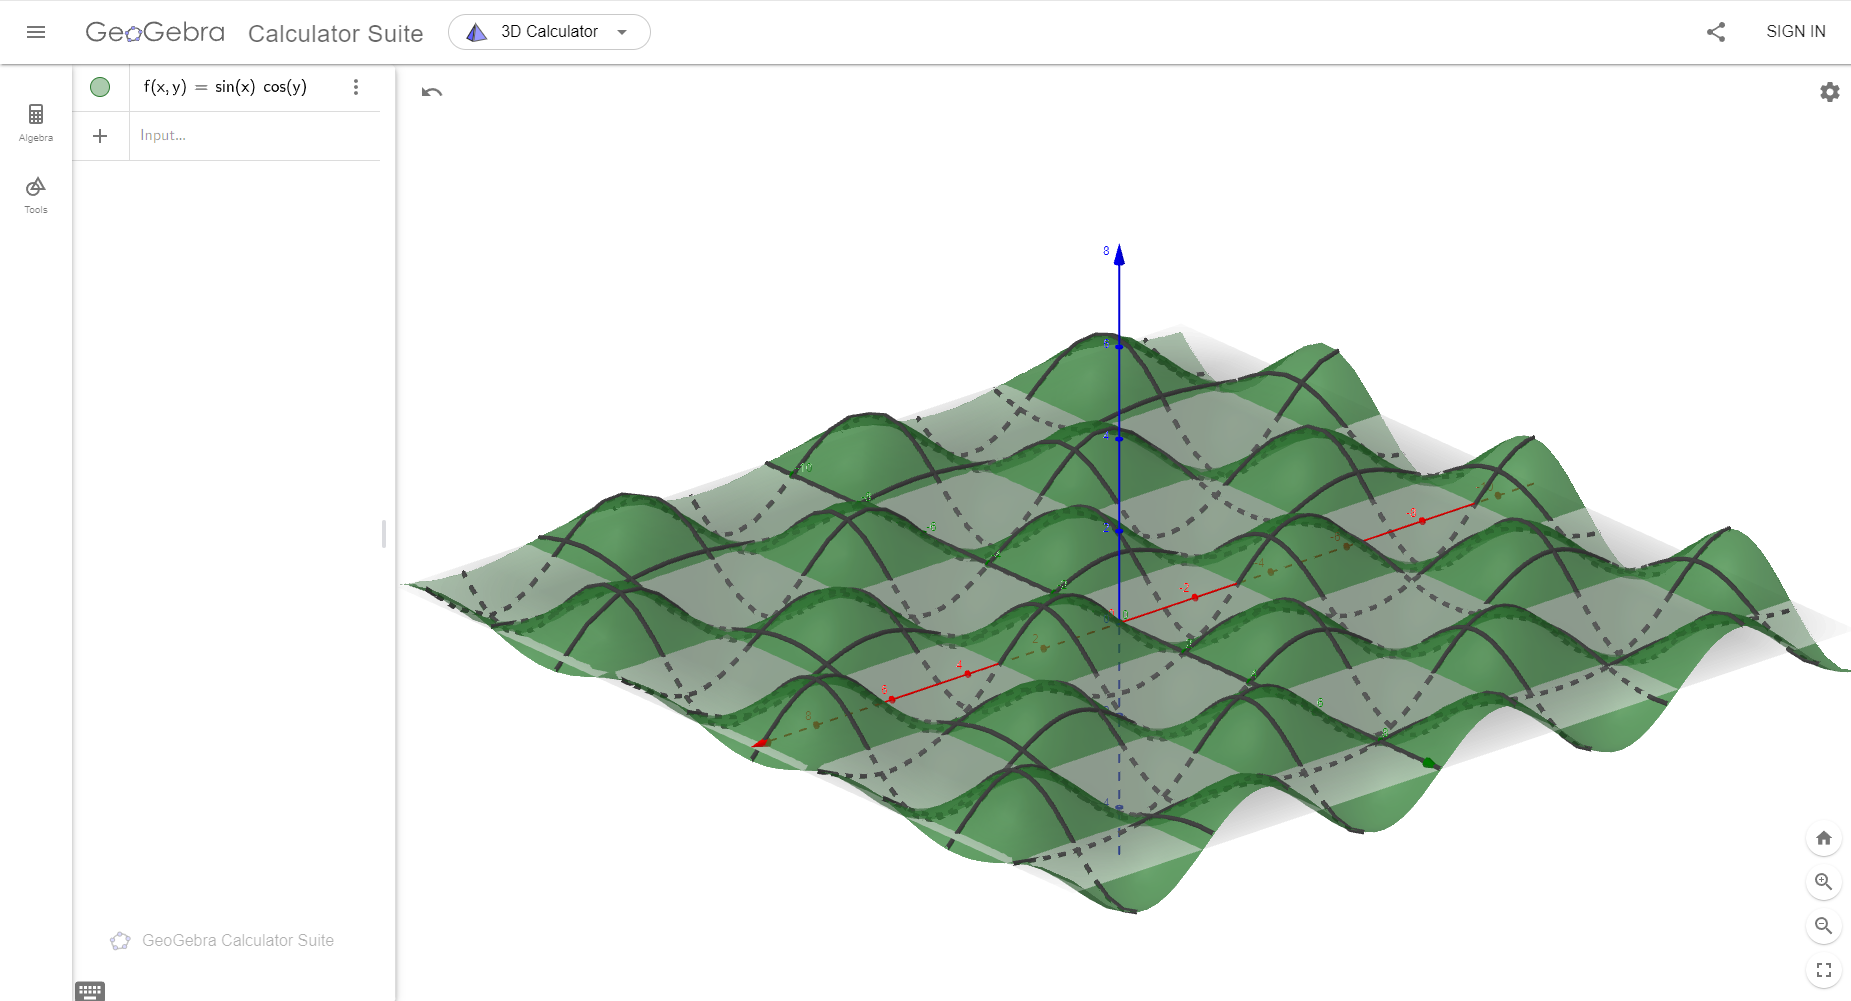
\includegraphics[scale=0.35]{fig/GeoBebra.png}
    \caption{Пример работы программы GeoGebra}
    \label{fig:24}
\end{figure}